\documentclass[10pt]{article}
\usepackage[polish]{babel}
\usepackage[utf8]{inputenc}
\usepackage[T1]{fontenc}
\usepackage{graphicx}
\usepackage[export]{adjustbox}
\graphicspath{ {./images/} }
\usepackage{amsmath}
\usepackage{amsfonts}
\usepackage{amssymb}
\usepackage[version=4]{mhchem}
\usepackage{stmaryrd}

\title{Zestaw 19 }

\author{}
\date{}


\newcommand\Varangle{\mathop{{<\!\!\!\!\!\text{\small)}}\:}\nolimits}

\begin{document}
\maketitle
\begin{center}

\includegraphics[max width=\textwidth]{2024_11_21_1c9a743c22bda6d33a9bg-1}
\end{center}

\begin{enumerate}
  \item Udowodnij, że ze środkowych dowolnego trójkąta zawsze można zbudować trójkąt i że pole tego trójkąta jest równe \(\frac{3}{4}\) pola wyjściowego trójkąta.
  \item Punt \(P\) leży na boku \(C D\) kwadratu \(A B C D\). Dwusieczna kąta \(B A P\) przecina odcinek \(B C\) w punkcie \(Q\). Udowodnij, że \(B Q+D P=A P\).
  \item Punkt \(P\) leży wewnątrz trójkąta \(A B C\), przy czym trójkąt \(A P C\) jest równoboczny. Niech \(\Varangle C B P=\alpha\) oraz \(\Varangle A B P=\beta\). Udowodnij, że z odcinków \(A B, P B\) i \(C B\) można zbudować trójkąt i\\
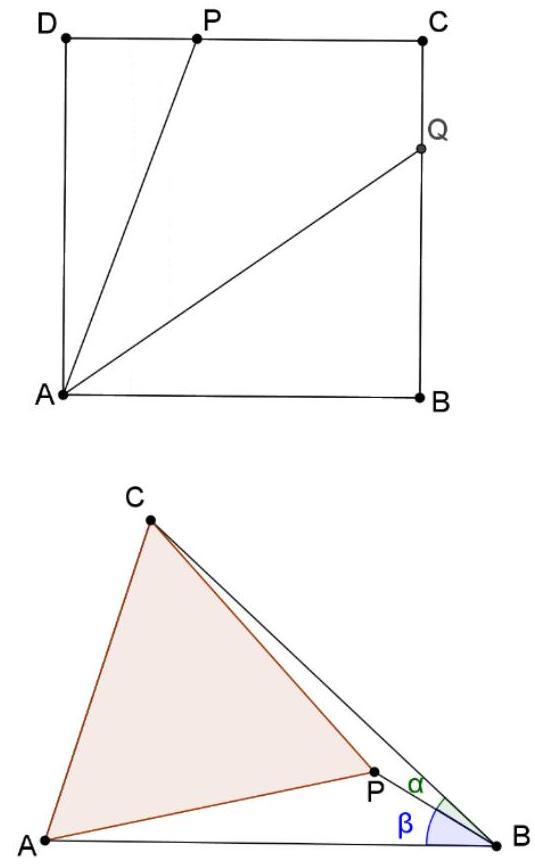
\includegraphics[max width=\textwidth, center]{2024_11_21_1c9a743c22bda6d33a9bg-1(1)}\\
wyznacz miary kątów tego trójkąta.
\end{enumerate}

\end{document}